% 
% Permission is granted to copy, distribute and/or modify this document
% under the terms of the GNU Free Documentation License, Version 1.2
% or any later version published by the Free Software Foundation;
% with no Invariant Sections, no Front-Cover Texts, and no Back-Cover
% Texts.  A copy of the license is included in the section entitled "GNU
% Free Documentation License".




%%%%%%%%%%%%%%%%%%%%%%%%%%%%%%%%%%%%%%%%%%%%%%%%%%%%%%%%%%%%%%%%%%%%%%%%%%%%%%%%%%%%%%%%%% 
\section{Reference Guide}

\subsection{Definition}

In probability theory, a \emph{compound Poisson distribution}  is the sum of a Poisson-distributed number of independent identically-distributed random variables. In the simplest cases, the result can be either a continuous or a discrete distribution.\\
If $N$ is a poisson distributed variable and if $(X_i)_i$ are identically distributed random variables that are mutually independent and also independent of $N$, then :

\begin{equation}
Y = \left( \displaystyle \sum_{i=1}^{N}X_i \right)\fcar{N\geq 1}
\end{equation}

is a compound Poisson distribution.\\

This module only focuses on  variables $X_i$ which are discrete, with finite range and integer values. We name this particular case the \emph{Integral Compound Poisson Distribution}. It implies that the compound Poisson distribution is also discrete, with finite range and integer values. Then, it allows the use of its generating function in order to evaluate its probability distribution.




\subsection{Distribution of the Integral Compound Poisson Distribution }\label{loiY}

Let us suppose that the variables $(X_i)_i$ are identically and independently distributed according to the $X$ distribution and that $N$ follows a Poisson distribution parameterised by $\lambda$.\\

The generating function of $N$ is, for $z\in[-1, 1]$ :
\begin{eqnarray}\label{PhiN}
\phi_{N}(z) = E[z^{N}] = e^{-\lambda(1-z)}
\end{eqnarray}

We show that the generating function of $Y$ writes :
\begin{eqnarray}
\phi_{Y}(z) = \phi_{N} \circ \phi_{X}(z)
\end{eqnarray}

Then, the probability distribution of $Y$ is derived from its generating function as follows :
\begin{eqnarray}
\forall n \in \mathbb{N}, \, \, \mathbb{P}(Y = n) = \displaystyle \left. \frac{1}{n!}\frac{d^{(n)}\phi_{Y}(z)}{dz^n } \right|_{z=0}
\end{eqnarray}


%%%%%%%%%%%%%%%%%%%%%%%%%%%%%%%%%%%%%%%%%%%%%%%%%%%%%%
\subsection{Algorithmic details}

The evaluation of the integral compound Poisson distribution is based on the previous results. The references \cite{Abate}, \cite{Stoer} and \cite{Feller} give more details on these results. We develop below some important points : the Cauchy's integral formula and the Poisson summation formula.

\subsubsection{Cauchy's integral formula}

In mathematics, Cauchy's integral formula, named after Augustin-Louis Cauchy, is a central statement in complex analysis. It expresses the fact that a holomorphic function defined on a disk is completely determined by its values on the boundary of the disk, and it provides integral formulas for all derivatives of a holomorphic function. Cauchy's celebrated formula shows that, in complex analysis, differentiation is equivalent to integration.\\

{\bf Cauchy Formula :} Suppose $U$ is an open subset of the complex plane $C$, $f : U \rightarrow C$ is a holomorphic function and the closed disk $D = \{ z : | z - z_0| = r\}$ is completely contained in $U$. Let $\gamma$ be the circle forming the boundary of $D$. Then for every a in the interior of $D$:

Let $f$ be a a holomorphic function on $\mathcal{U}$  an open subset of the complex plane $\mathbb{C}$, $K$ a compact of $\mathcal{U}$ completely contained in $\mathcal{U}$ and $\Gamma$ its boundary. Then for every $z_0 \in K-\Gamma$, we have : 
\begin{eqnarray}\label{forCauchy}
 f(z_0).1_{\Gamma}(z_0)= \displaystyle \frac{1}{2i\pi}\int_{\Gamma} \frac{f(u)}{u-z_0}du
\end{eqnarray}
where $1_{\Gamma}(z_0) = \int_{\Gamma} \frac{1}{u-z_0}du$.\\

With $\Gamma = Circle(0,r)$ and $z_0 = 0$, then the relation  (\ref{forCauchy}) writes : 
\begin{eqnarray}\label{f20}
f(0) = \displaystyle \frac{1}{2i\pi}\int_{\Gamma} \frac{f(u)}{u}du
\end{eqnarray}
and we show that : 
\begin{eqnarray}\label{fn20}
f^n(0) = \displaystyle \frac{n!}{2i\pi}\int_{\Gamma} \frac{f(u)}{u^{n+1}}du
\end{eqnarray}

Then, with a proper parametrisation of the circle, we have: 
\begin{eqnarray}\label{fn20Pol}
f^n(0) = \displaystyle \frac{n!}{2\pi r^n}\int_{0}^{2\pi} f\left(re^{i\theta}\right)e^{-in\theta} d\theta
\end{eqnarray}


The relation (\ref{fn20Pol}) applied to the generating function $\phi$ of $Y$ writes :
\begin{eqnarray}\label{pnCauchy}
p_n = \displaystyle \frac{1}{2\pi r^n}\int_{0}^{2\pi} \phi\left(re^{i\theta}\right)e^{-in\theta} d\theta
\end{eqnarray}



\subsubsection{Poisson summation formula}

In mathematics, the Poisson summation formula is an equation that allows us to relate the Fourier series coefficients of the periodic summation of a function to values of the function's continuous Fourier transform. Consequently, the periodic summation of a function is completely defined by discrete samples of the original function's Fourier transform. And conversely, the periodic summation of a function's Fourier transform is completely defined by discrete samples of the original function. The Poisson summation formula was discovered by Siméon Denis Poisson and is sometimes called Poisson resummation.\\

The relation (\ref{pnCauchy}) requires the Poisson summation formula.\\

Let  $g$ be a function from $\mathbb{R}$ into $\mathbb{R}$ as:
\begin{eqnarray}\label{g2u}
g(u) = \sum_{k=-\infty}^{+\infty} a_k e^{iku}
\end{eqnarray}
then $a_n$ writes :
\begin{eqnarray}\label{an}
a_n = \frac{1}{2\pi}\int_{0}^{2\pi} g(u)e^{-in\theta} d\theta
\end{eqnarray}
If we consider the periodic suite :
\begin{eqnarray}\label{anp}
a_n^p =  \sum_{k=-\infty}^{+\infty} a_{n+km}
\end{eqnarray}
for a given integer $m$, we show that $a_n^p$ can write as : 
\begin{eqnarray}\label{anp2}
a_n^p =  \displaystyle \frac{1}{m} \sum_{k=0}^{m-1} g\left(\frac{2\pi k}{m}\right)e^{-\frac{2i\pi kn}{m}}
\end{eqnarray}
whioch leads to the  {\bf Poisson summation formula :}
\begin{eqnarray}\label{forSomPoisson}
\sum_{k=0}^{m-1} g\left(\frac{2\pi k}{m}\right)e^{-\frac{2i\pi kn}{m}} = m \sum_{k=-\infty}^{+\infty}a_{n+km}
\end{eqnarray}

The figure \ref{FigAnp} gives an illustration of the periodic suite $a_n$.

\begin{figure}[hbtp]
     \begin{center}
      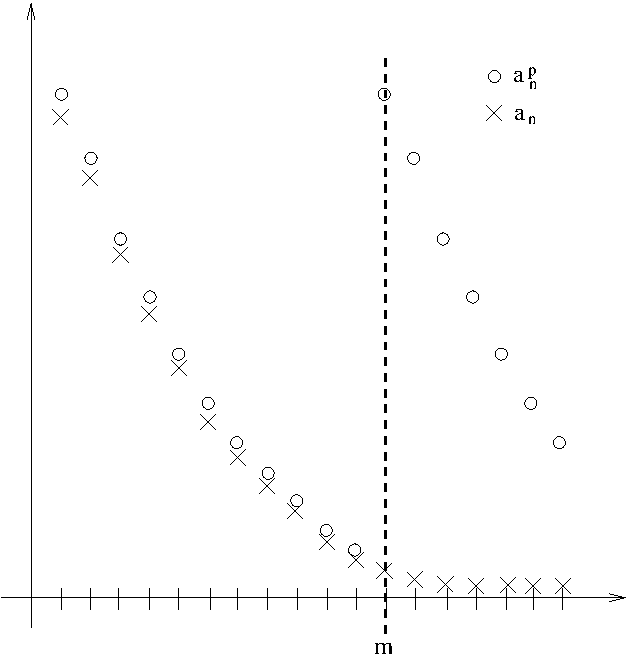
\includegraphics[width=8cm]{figAnp.pdf} 
      \caption{Periodic suite $a_n$.}
      \label{FigAnp}
    \end{center}
 \end{figure}





As the function $g$ writes as a convergent serie (\ref{g2u}), $|a_k| \underset{k \rightarrow +\infty}{\rightarrow} 0$. Then if we take $m$ great enough, we obtain the following approximation : 
\begin{eqnarray}\label{anpApprox}
a_n^p  =  \sum_{k=-\infty}^{+\infty} a_{n+km} \simeq a_n
\end{eqnarray}

In our probabilistic context, the function $g$ is : 
\begin{eqnarray}\label{cadreProb}
g(u) = \phi\left(re^{iu}\right) = \sum_{k=0}^{+\infty}p_k r^k e^{iku}
\end{eqnarray}
wich leads to the expression (\ref{g2u}) with
\begin{equation}\label{cadreProb2}
\left\{
\begin{array}{ll}
  a_k = 0, & \forall k<0 \\
  a_k = p_kr^k & \forall k \geq 0
\end{array}
\right.
\end{equation}

The relation (\ref{forSomPoisson}) writes, for $n < m$ and for the function $g$ defined in (\ref{cadreProb2})  :
\begin{eqnarray}\label{forSomPoissonG}
m \sum_{k=0}^{+\infty}a_{n+km} = \sum_{k=0}^{m-1} g\left(\frac{2\pi k}{m}\right)e^{-\frac{2i\pi kn}{m}}
\end{eqnarray}
By isolating the term $a_n$ in (\ref{forSomPoissonG}), we have : 
\begin{eqnarray}\label{termeAn}
a_n = \displaystyle \frac{1}{m} \sum_{k=0}^{m-1} g\left(\frac{2\pi k}{m}\right)e^{-\frac{2i\pi kn}{m}} - \sum_{k=1}^{+\infty}a_{n+km}
\end{eqnarray}
which, within the probabilistic context of (\ref{cadreProb}) and (\ref{cadreProb2}) leads to the expression of $p_n$ : 
\begin{eqnarray}\label{pnApprox}
p_n = \displaystyle \frac{1}{mr^n} \sum_{k=0}^{m-1} \phi\left(re^{\frac{2i\pi k}{m}}\right) e^{-\frac{2i\pi kn}{m}} - e_d
\end{eqnarray}
where $e_d$ is the approximation error done if we neglige this term in (\ref{pnApprox}). This error writes : 
\begin{eqnarray}\label{ed}
e_d = \displaystyle \sum_{k=1}^{+\infty}p_{n+km}r^{km}
\end{eqnarray}
and can be bounded, for $0 < r < 1$ : 
\begin{eqnarray}\label{edEncadr}
0 < e_d \leq  \sum_{k=1}^{+\infty}r^{km} = \displaystyle \frac{r^m}{1-r^m}
\end{eqnarray}
Thus, the precision of the evaluation of $p_n$ is given by the choice of the couple $(m,r)$.\\

We have the following final result : 
\begin{eqnarray}\label{pnApprox2}
\forall n < m, \, \, p_n \simeq \hat{p}_n = \displaystyle \frac{1}{mr^n} \sum_{k=0}^{m-1} \phi\left(re^{\frac{2i\pi k}{m}}\right) e^{-\frac{2i\pi kn}{m}}
\end{eqnarray}
where
\begin{eqnarray}\label{erreurRel}
\displaystyle |p_n - \hat{p}_n | \leq  \frac{r^m}{1-r^m}
\end{eqnarray}


\subsubsection{Fast Fourier Transform (FFT)}

In order to optimize the numerical evaluation of the $(\hat{p}_n)_n$ given in (\ref{pnApprox2}), it is recommended to use the Fast Fourier Transform (FFT) which evaluates simultaneously the values $(p_0, \hdots, p_{m-1})$ with an optimised cost.\\

The relation (\ref{pnApprox2}) presents $mr^np_n$ as the result of a discrete Fast Fourier Transform of the suite $\left(\phi\left(re^{\frac{2i\pi k}{m}}\right)\right)_{k \geq 0}$.\\
If we chose $m$ as a power of 2, we can evaluate $(p_0, \hdots, p_{m-1})$ thanks to the FFT. The algorithmic cost is no more $\mathcal{O}(m^2)$ but  $\mathcal{O}(m\log m)$.





%\subsection{References}


\addcontentsline{toc}{subsection}{Bibliographie}
\begin{thebibliography}{9}
  \bibitem {Abate} J. Abate, W. Whitt,
     \emph{The Fourier-series method for inverting transforms of probability distributions.}
     Queueing Systems, feb. 1991.
  \bibitem {Stoer}J. Stoer, R. Bulirsch,
     \emph{Introduction to numerical analysis.}
     Springer, Third Edition, 2002.
  \bibitem {Feller} W. Feller,
     \emph{Introduction to probability theory and its application.}
     Wiley, Second Edition, vol 2, 1971.
\end{thebibliography}



